% Backup slides (not counted in the talk).
\begin{frame}{Backup: layer \ding{172}, all methods and strategies}
  \centering
  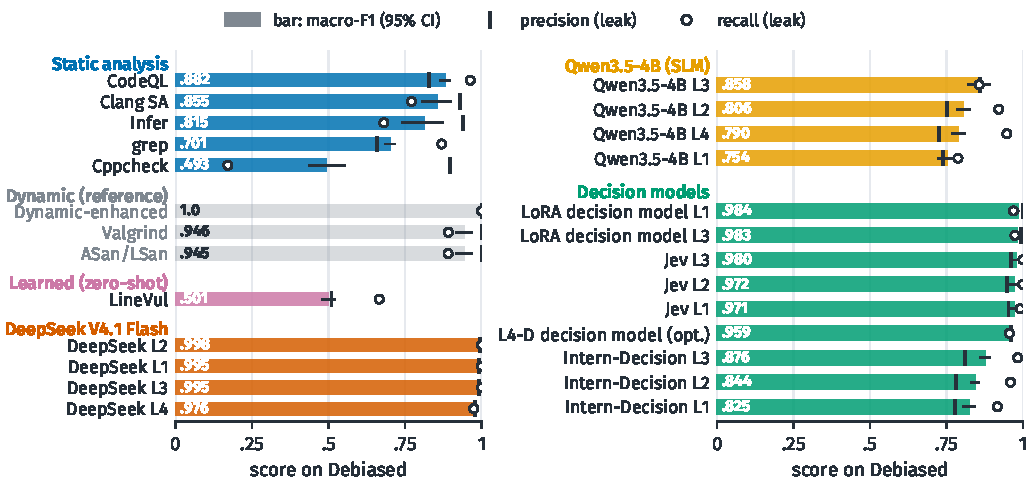
\includegraphics[width=\linewidth,height=0.86\textheight,keepaspectratio]{figures/prf1_full.pdf}
\end{frame}

% ------------------------------------------------------------------------------
\begin{frame}{Backup: robustness, all methods and strategies}
  \centering
  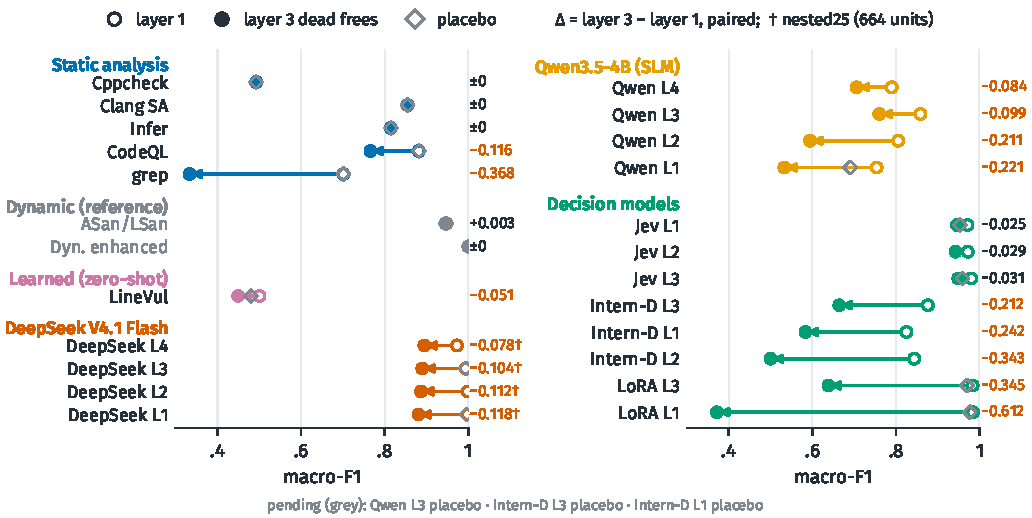
\includegraphics[width=\linewidth,height=0.83\textheight,keepaspectratio]{figures/robustness_full.pdf}
\end{frame}

% ------------------------------------------------------------------------------
\begin{frame}{Backup: where each method fails, by flow category}
  \centering
  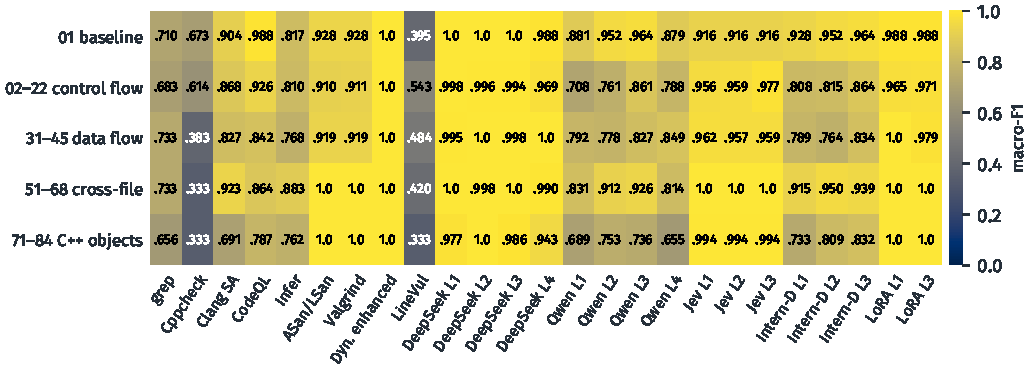
\includegraphics[width=\linewidth,height=0.76\textheight,keepaspectratio]{figures/heatmap.pdf}
  \\[2pt]{\scriptsize Macro-F1 on layer \ding{172}, eval set, per Juliet flow-variant group.\par}
\end{frame}

% ------------------------------------------------------------------------------
\begin{frame}{Backup: by leak mechanism and good-unit kind}
  \centering
  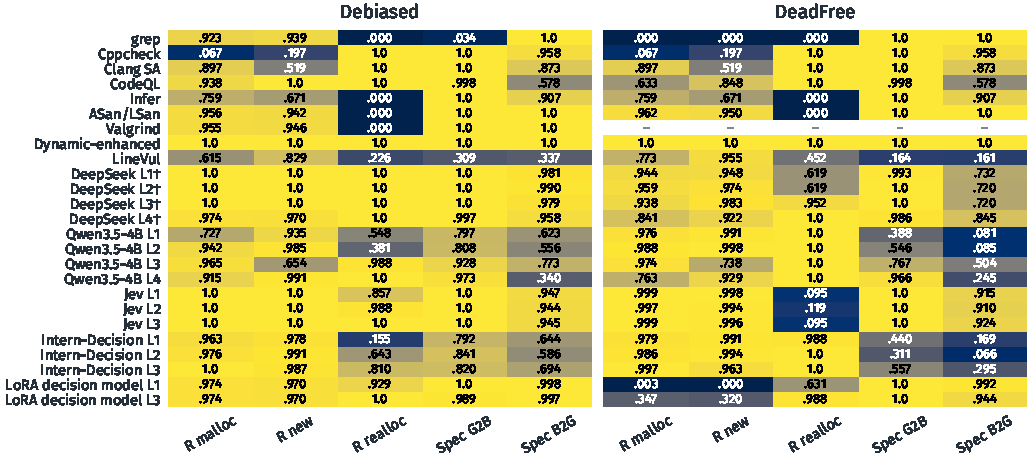
\includegraphics[width=\linewidth,height=0.80\textheight,keepaspectratio]{figures/mechanism.pdf}
  \\[2pt]{\scriptsize Leak recall per mechanism (bad units); specificity per good kind (G2B / B2G). Layer \ding{172} vs \ding{174}.\par}
\end{frame}

% ------------------------------------------------------------------------------
\begin{frame}{Backup: repeat agreement and merged vs unmerged LoRA}
  \begin{columns}[T]
    \begin{column}{0.48\textwidth}
      {\small Same prompt, 3 runs (layer \ding{172})\\[2pt]
      % generated by figures/make_figures.py -- do not edit
\begin{tabular}{@{}lrr@{}}
\toprule
Model & units & all 3 runs agree \\
\midrule
DeepSeek L1 & 200 & 1.000 \\
DeepSeek L2 & 200 & 1.000 \\
DeepSeek L3 & 200 & 0.990 \\
Jev L1 & 2,656 & 0.989 \\
Jev L2 & 2,656 & 0.996 \\
Jev L3 & 2,656 & 0.995 \\
Qwen L1 & & \textit{pending} \\
Qwen L2 & & \textit{pending} \\
Qwen L3 & & \textit{pending} \\
\bottomrule
\end{tabular}
\par}
    \end{column}
    \begin{column}{0.48\textwidth}
      \begin{itemize}\small
        \item Reported LoRA = adapters \textbf{merged} into BF16 weights; 3 held-out folds combined
        \item Unmerged adapters, layer \ding{172}: L1 \res{lora_unmerged_L1-layer1}{macro}, L3 \res{lora_unmerged_L3-layer1}{macro}
        \item Held-out predictions that differ: \res{x}{unmerged_flips_L1} (L1), \res{x}{unmerged_flips_L3} (L3) of 2,656
        \item Scores differ only by BF16 rounding of large logits ($|s|\approx15$--$40$)
      \end{itemize}
    \end{column}
  \end{columns}
\end{frame}

% ------------------------------------------------------------------------------
\begin{frame}{Backup: CodeQL batching artifact}
  \begin{itemize}
    \item CodeQL builds one database per \textbf{50 units} (7.36\,s $\to$ 0.32\,s per unit)
    \item \code{\_08} units each define helpers \code{staticReturnsTrue/False}; they are not renamed per unit
    \item In a shared database, CodeQL cannot resolve which helper a guard calls: ``may not be freed'' fires
    \item Result: \textbf{4} extra false positives on eval good units (per-unit runs are clean)
    \item Not corrected: the configuration was frozen before eval. Fix = rename all non-\code{main} functions per unit
  \end{itemize}
\end{frame}

% ------------------------------------------------------------------------------
\begin{frame}{Backup: cost of every API run}
  \begin{columns}[T]
    \begin{column}{0.60\textwidth}
      {\scriptsize% generated by figures/make_figures.py from juliet_full/llm/ledger.jsonl
\begin{tabular}{@{}llrr@{}}
\toprule
Provider & Runs & calls & cost \\
\midrule
DeepSeek & Debiased (incl.\ dev, repeats, latency) & 13,877 & \textyen5.46 \\
DeepSeek & DeadFree & 11,824 & \textyen5.37 \\
DeepSeek & Placebo & 1,328 & \textyen0.42 \\
DeepSeek & Original & 664 & \textyen0.30 \\
DeepSeek & demo & 30 & \textyen0.01 \\
\textbf{DeepSeek} & \textbf{total} & \textbf{27,723} & \textbf{\textyen11.57} \\
\midrule
Jev & Debiased (incl.\ dev, repeats, latency) & 27,420 & \$1.23 \\
Jev & DeadFree & 8,868 & \$0.42 \\
Jev & Placebo & 5,312 & \$0.20 \\
Jev & Original & 2,656 & \$0.10 \\
Jev & demo & 11 & \$0.00 \\
\textbf{Jev} & \textbf{total} & \textbf{44,267} & \textbf{\$1.95} \\
\bottomrule
\end{tabular}
\par}
    \end{column}
    \begin{column}{0.37\textwidth}
      \begin{itemize}\small
        \item User cap: DeepSeek $\le$ \textyen10; client hard stop at \textyen9.5
        \item Total: \textyen\res{x}{cost_deepseek} and \$\res{x}{cost_jev}, from the shared ledger
        \item This is why DeepSeek layer \ding{174}, placebo and original use nested25 (664 units)
        \item Local models: 2$\times$RTX 3090, no API cost
      \end{itemize}
    \end{column}
  \end{columns}
\end{frame}

% ------------------------------------------------------------------------------
\begin{frame}{Backup: latency at concurrency 1 (Pareto x-axis)}
  \centering
  {\tiny\renewcommand{\arraystretch}{0.92}\resizebox{\linewidth}{!}{% generated by figures/make_figures.py from figures/latency_c1.csv
\begin{tabular}{@{}lrl@{}}
\toprule
Method & s / unit & Source (juliet\_full/\ldots); note \\
\midrule
grep & <0.001 & \texttt{static/results/grep\_v0/layer1/lat300\_c1.jsonl}; median of 300 units (1 µs) \\
Cppcheck & 0.008 & \texttt{static\_stage2.md}; lat300 per unit \\
Clang SA & 0.018 & \texttt{static\_stage2.md}; lat300 per unit \\
Infer & 0.278 & \texttt{static\_stage2.md}; lat300 per unit \\
CodeQL & 7.36 & \texttt{static\_stage2.md}; per unit: database creation + queries (20 units) \\
CodeQL (50 per database) & 0.318 & \texttt{static\_stage2.md}; 50 units per database; amortized (hollow marker) \\
LineVul (GPU) & 0.006 & \texttt{gpu\_stage1.md}; GPU (RTX 3090) \\
LineVul (CPU) & 0.088 & \texttt{gpu/results/linevul\_cpu/layer1/lat300\_cpu\_quiet.jsonl}; CPU 6 threads; quiet; median of 300 \\
DeepSeek L1 & 0.721 & \texttt{llm\_stage2b.md}; lat300\_c1\_L1 at load ~21; quiet 0.640 s on 30 dev units (llm\_stage2a) \\
Qwen L1 & 0.665 & \texttt{gpu\_stage1.md}; vLLM from dell; 30 requests \\
Jev L1 & 0.961 & \texttt{llm\_stage2b.md}; lat300\_c1\_L1 at load ~22 \\
Intern-D L1 & 0.083 & \texttt{gpu\_stage1.md}; /decide read-out from dell (82.7 ms) \\
LoRA L1 & 0.105 & \texttt{decision\_ft\_stage2.md}; latency300; dell end-to-end \\
LoRA L3 & 0.133 & \texttt{decision\_ft\_stage2.md}; latency300; dell end-to-end \\
ASan/LSan & 0.134 & \texttt{data\_stage4.md}; lat300\_c1; compile included \\
Valgrind & 0.407 & \texttt{data\_stage4.md}; lat300\_c1; compile included \\
Dyn. enhanced & 1.194 & \texttt{data\_stage4.md}; lat300\_c1; compile included \\
\bottomrule
\end{tabular}
}\par}
  \vfill
  {\scriptsize Never \texttt{latency\_s} from bulk runs. Source table: \texttt{figures/latency\_c1.csv}.\par}
\end{frame}

% ------------------------------------------------------------------------------
\begin{frame}{Backup: are the labels still right? Compile and run every unit}
  \begin{columns}[T]
    \begin{column}{0.46\textwidth}
      \begin{itemize}\small
        \item gcc and clang compile \textbf{3,316 / 3,316} units in every layer
        \item No good unit is flagged by ASan/LSan or the enhanced dynamic run
        \item Labels are never changed; disagreements are explained, not relabelled
      \end{itemize}
    \end{column}
    \begin{column}{0.51\textwidth}
      {\footnotesize Enhanced dynamic run: what it takes to catch the 1,658 bad units\\[2pt]
      \begin{tabular}{@{}lr@{}}
        \toprule
        Needed & units \\
        \midrule
        plain run, every seed & 1,448 \\
        some seeds only (variant 12, random) & 34 \\
        \texttt{use\_globals=0} (globals at exit) & 68 \\
        \texttt{realloc} failure injected & 108 \\
        \bottomrule
      \end{tabular}}
    \end{column}
  \end{columns}
\end{frame}

% ------------------------------------------------------------------------------
\begin{frame}{Backup: why dynamic tools are a reference line, not a competitor}
  \begin{itemize}
    \item Plain ASan/LSan: precision 1.000, macro-F1 \res{asan_lsan-layer1}{macro} on layer \ding{172}
    \item Misses: \code{realloc} failure 0/84 eval bad units; global still reachable at exit (variants 45/68);
          random branch not taken (variant 12)
    \item We run LSan with \code{use\_stacks=0}: default options miss 175 more bad units (stale \code{-O0} stack slots)
    \item Enhanced (seeds, \code{use\_globals=0}, failure injection) reaches \res{dynamic_enhanced-layer1}{macro}, but
          only because we know which input and which fault to inject
    \item They need a build, a run and the right input: a different question from reading code
  \end{itemize}
\end{frame}

% ------------------------------------------------------------------------------
\begin{frame}[fragile]{Backup: demo replay}
  \begin{columns}[T]
    \begin{column}{0.56\textwidth}
      {\small Stage unit \texttt{strdup\_char\_01}, bad, after the edit:\par}
\begin{lstlisting}[style=unit]
static const int sym_61 = 4; /* added */
void sym_0() {
  char * data;
  data = NULL;
  {
    char myString[] = "myString";
    data = strdup(myString);
    printLine(data);
  }
  if(sym_61 > 4) {  /* added */
    free(data);     /* never runs */
  }
}
\end{lstlisting}
    \end{column}
    \begin{column}{0.40\textwidth}
      \begin{itemize}\small
        \item Fallback if the network or GPU server fails:\\
              {\scriptsize\texttt{demo.py --replay}\\ \texttt{recordings/stage\_dryrun.json}}
        \item Dry run cost: \textyen\res{x}{demo_cny} DeepSeek, \$\res{x}{demo_usd} Jev
        \item Fooled: grep, LoRA L1/L3. Robust: Clang SA, DeepSeek L1/L3, Jev
      \end{itemize}
    \end{column}
  \end{columns}
\end{frame}

% ------------------------------------------------------------------------------
\begin{frame}{Backup: earlier SecVulEval study}
  \begin{itemize}
    \item Proposal tier A: real CVE functions from SecVulEval (Ahmed et al., AIware'26)
    \item Pair task (vulnerable vs patched): MiMo's single-order accuracy of 86.7\% looked strong
    \item Swapping the order: MiMo 74.44\%, DeepSeek 61.67\% (below a length heuristic)
    \item Same lesson as Juliet: check the benchmark before ranking models; full write-up goes in the report appendix
  \end{itemize}
\end{frame}

% ------------------------------------------------------------------------------
% generated by figures/make_figures.py -- do not edit (input outside a frame)
\begin{frame}{Backup: result files used (1/5)}
\centering
{\tiny\renewcommand{\arraystretch}{0.85}\setlength{\tabcolsep}{4pt}\begin{tabular}{@{}llll@{}}
\toprule
Method & Layer & Run file (juliet\_full/\ldots; r = results) & sha256 \\
\midrule
grep & Debiased & \texttt{static/r/grep\_v0/layer1/full\_v1.jsonl} & \texttt{9a425c0e} \\
grep & DeadFree & \texttt{static/r/grep\_v0/layer3/full\_v1.jsonl} & \texttt{a0a26ccd} \\
grep & Placebo & \texttt{static/r/grep\_v0/placebo/full\_v1.jsonl} & \texttt{0e7c92ed} \\
grep & Original & \texttt{static/r/grep\_v0/original/full\_v1.jsonl} & \texttt{5c3bf9ea} \\
Cppcheck & Debiased & \texttt{static/r/cppcheck/layer1/full\_v2.jsonl} & \texttt{b3ae0a0e} \\
Cppcheck & DeadFree & \texttt{static/r/cppcheck/layer3/full\_v1.jsonl} & \texttt{3bd521e3} \\
Cppcheck & Placebo & \texttt{static/r/cppcheck/placebo/full\_v1.jsonl} & \texttt{aade3fed} \\
Cppcheck & Original & \texttt{static/r/cppcheck/original/full\_v1.jsonl} & \texttt{26245ae1} \\
Clang SA & Debiased & \texttt{static/r/clang\_sa/layer1/full\_v2.jsonl} & \texttt{9fff5bc7} \\
Clang SA & DeadFree & \texttt{static/r/clang\_sa/layer3/full\_v1.jsonl} & \texttt{29c2c3cb} \\
Clang SA & Placebo & \texttt{static/r/clang\_sa/placebo/full\_v1.jsonl} & \texttt{a031bf11} \\
Clang SA & Original & \texttt{static/r/clang\_sa/original/full\_v1.jsonl} & \texttt{d48a49c1} \\
CodeQL & Debiased & \texttt{static/r/codeql/layer1/full\_batch50\_merged.jsonl} & \texttt{1e41db0c} \\
CodeQL & DeadFree & \texttt{static/r/codeql/layer3/full\_batch50.jsonl} & \texttt{26cf528a} \\
CodeQL & Placebo & \texttt{static/r/codeql/placebo/full\_batch50.jsonl} & \texttt{203de4f7} \\
CodeQL & Original & \texttt{static/r/codeql/original/full\_batch50.jsonl} & \texttt{e6133458} \\
Infer & Debiased & \texttt{static/r/infer/layer1/full\_per\_file\_merged.jsonl} & \texttt{ba59f70d} \\
Infer & DeadFree & \texttt{static/r/infer/layer3/full\_per\_file.jsonl} & \texttt{69dda662} \\
Infer & Placebo & \texttt{static/r/infer/placebo/full\_per\_file.jsonl} & \texttt{161f789c} \\
Infer & Original & \texttt{static/r/infer/original/full\_per\_file.jsonl} & \texttt{36074229} \\
LineVul & Debiased & \texttt{gpu/r/linevul\_gpu/layer1/deveval\_v1.jsonl} & \texttt{8bc1535e} \\
LineVul & DeadFree & \texttt{gpu/r/linevul\_gpu/layer3/all\_v1.jsonl} & \texttt{2bf0d6ab} \\
\bottomrule
\end{tabular}\par}
\vfill
{\scriptsize Scored with \texttt{juliet\_full/analysis/score.py} on the eval set (2,656 units); \texttt{figures/make\_figures.py}.\par}
\end{frame}
\begin{frame}{Backup: result files used (2/5)}
\centering
{\tiny\renewcommand{\arraystretch}{0.85}\setlength{\tabcolsep}{4pt}\begin{tabular}{@{}llll@{}}
\toprule
Method & Layer & Run file (juliet\_full/\ldots; r = results) & sha256 \\
\midrule
LineVul & Placebo & \texttt{gpu/r/linevul\_gpu/placebo/all\_v1.jsonl} & \texttt{19529812} \\
LineVul & Original & \texttt{gpu/r/linevul\_gpu/original/all\_v1.jsonl} & \texttt{7d2e9b26} \\
ASan/LSan & Debiased & \texttt{data/r/asan\_lsan/layer1/full\_v1.jsonl} & \texttt{684c4195} \\
ASan/LSan & DeadFree & \texttt{data/r/asan\_lsan/stress/full\_v1.jsonl} & \texttt{97a9eb40} \\
ASan/LSan & Placebo & \texttt{data/r/asan\_lsan/placebo/full\_v1.jsonl} & \texttt{9eda685e} \\
ASan/LSan & Original & \texttt{data/r/asan\_lsan/original/full\_v1.jsonl} & \texttt{8945394e} \\
Valgrind & Debiased & \texttt{data/r/valgrind/layer1/full\_v1.jsonl} & \texttt{fb6481b7} \\
Dynamic-enhanced & Debiased & \texttt{data/r/dynamic\_enhanced/layer1/full\_v1.jsonl} & \texttt{758daeac} \\
Dynamic-enhanced & DeadFree & \texttt{data/r/dynamic\_enhanced/stress/full\_v1.jsonl} & \texttt{cf47c76c} \\
Dynamic-enhanced & Placebo & \texttt{data/r/dynamic\_enhanced/placebo/full\_v1.jsonl} & \texttt{181e81b2} \\
DeepSeek L1 & Debiased & \texttt{llm/r/deepseek\_flash/layer1/eval\_L1\_r1.jsonl} & \texttt{912db2f0} \\
DeepSeek L1 & DeadFree & \texttt{llm/r/deepseek\_flash/layer3/l3\_n25\_L1\_r1.jsonl} & \texttt{376d1393} \\
DeepSeek L1 & Placebo & \texttt{llm/r/deepseek\_flash/placebo/pl\_n25\_L1\_r1.jsonl} & \texttt{6480450e} \\
DeepSeek L1 & Original & \texttt{llm/r/deepseek\_flash/original/orig\_n25\_L1\_r1.jsonl} & \texttt{034fdebe} \\
DeepSeek L2 & Debiased & \texttt{llm/r/deepseek\_flash/layer1/eval\_L2\_r1.jsonl} & \texttt{ee6c51f4} \\
DeepSeek L2 & DeadFree & \texttt{llm/r/deepseek\_flash/layer3/l3\_n25\_L2\_r1.jsonl} & \texttt{369a2a1f} \\
DeepSeek L3 & Debiased & \texttt{llm/r/deepseek\_flash/layer1/eval\_L3\_r1.jsonl} & \texttt{4bf6db11} \\
DeepSeek L3 & DeadFree & \texttt{llm/r/deepseek\_flash/layer3/l3\_n25\_L3\_r1.jsonl} & \texttt{6f396914} \\
DeepSeek L3 & Placebo & \texttt{llm/r/deepseek\_flash/placebo/pl\_n25\_L3\_r1.jsonl} & \texttt{c56b0f67} \\
DeepSeek L4 & Debiased & \texttt{llm/r/deepseek\_flash/layer1/eval\_L4\_r1.jsonl} & \texttt{0af89897} \\
DeepSeek L4 & DeadFree & \texttt{llm/r/deepseek\_flash/layer3/l3\_n25\_L4\_r1.jsonl} & \texttt{37d32759} \\
Qwen3.5-4B L1 & Debiased & \texttt{llm/r/qwen3\_5\_4b/layer1/eval\_L1\_r1.jsonl} & \texttt{0c952905} \\
\bottomrule
\end{tabular}\par}
\vfill
{\scriptsize Scored with \texttt{juliet\_full/analysis/score.py} on the eval set (2,656 units); \texttt{figures/make\_figures.py}.\par}
\end{frame}
\begin{frame}{Backup: result files used (3/5)}
\centering
{\tiny\renewcommand{\arraystretch}{0.85}\setlength{\tabcolsep}{4pt}\begin{tabular}{@{}llll@{}}
\toprule
Method & Layer & Run file (juliet\_full/\ldots; r = results) & sha256 \\
\midrule
Qwen3.5-4B L1 & DeadFree & \texttt{llm/r/qwen3\_5\_4b/layer3/l3\_eval\_L1\_r1.jsonl} & \texttt{c9e21163} \\
Qwen3.5-4B L1 & Placebo & \texttt{llm/r/qwen3\_5\_4b/placebo/pl\_eval\_L1\_r1.jsonl} & \texttt{41998d19} \\
Qwen3.5-4B L1 & Original & \texttt{llm/r/qwen3\_5\_4b/original/orig\_eval\_L1\_r1.jsonl} & \texttt{d0a08dbd} \\
Qwen3.5-4B L2 & Debiased & \texttt{llm/r/qwen3\_5\_4b/layer1/eval\_L2\_r1.jsonl} & \texttt{43c641b2} \\
Qwen3.5-4B L2 & DeadFree & \texttt{llm/r/qwen3\_5\_4b/layer3/l3\_eval\_L2\_r1.jsonl} & \texttt{337dc906} \\
Qwen3.5-4B L3 & Debiased & \texttt{llm/r/qwen3\_5\_4b/layer1/eval\_L3\_r1.jsonl} & \texttt{d0d1469a} \\
Qwen3.5-4B L3 & DeadFree & \texttt{llm/r/qwen3\_5\_4b/layer3/l3\_eval\_L3\_r1.jsonl} & \texttt{3c3ddd18} \\
Qwen3.5-4B L3 & Placebo & \texttt{llm/r/qwen3\_5\_4b/placebo/pl\_eval\_L3\_r1.jsonl} & \texttt{9fdeb3fd} \\
Qwen3.5-4B L4 & Debiased & \texttt{llm/r/qwen3\_5\_4b/layer1/eval\_L4\_r1.jsonl} & \texttt{266a3cc9} \\
Qwen3.5-4B L4 & DeadFree & \texttt{llm/r/qwen3\_5\_4b/layer3/l3\_eval\_L4\_r1.jsonl} & \texttt{5c2708a1} \\
Jev L1 & Debiased & \texttt{llm/r/jev/layer1/eval\_L1\_r1.jsonl} & \texttt{b0a4576e} \\
Jev L1 & DeadFree & \texttt{llm/r/jev/layer3/l3\_eval\_L1\_r1.jsonl} & \texttt{59fe6079} \\
Jev L1 & Placebo & \texttt{llm/r/jev/placebo/pl\_eval\_L1\_r1.jsonl} & \texttt{77d9bfce} \\
Jev L1 & Original & \texttt{llm/r/jev/original/orig\_eval\_L1\_r1.jsonl} & \texttt{6d574be5} \\
Jev L2 & Debiased & \texttt{llm/r/jev/layer1/eval\_L2\_r1.jsonl} & \texttt{ca0bf9e1} \\
Jev L2 & DeadFree & \texttt{llm/r/jev/layer3/l3\_eval\_L2\_r1.jsonl} & \texttt{fbe5242d} \\
Jev L3 & Debiased & \texttt{llm/r/jev/layer1/eval\_L3\_r1.jsonl} & \texttt{a5977265} \\
Jev L3 & DeadFree & \texttt{llm/r/jev/layer3/l3\_eval\_L3\_r1.jsonl} & \texttt{cb498e82} \\
Jev L3 & Placebo & \texttt{llm/r/jev/placebo/pl\_eval\_L3\_r1.jsonl} & \texttt{f5c6f04e} \\
Intern-Decision L1 & Debiased & \texttt{gpu/r/intern\_decision/layer1/eval\_L1\_r1.jsonl} & \texttt{f1e87ff7} \\
Intern-Decision L1 & DeadFree & \texttt{gpu/r/intern\_decision/layer3/l3\_eval\_L1\_r1.jsonl} & \texttt{7a52bf2f} \\
Intern-Decision L1 & Placebo & \texttt{gpu/r/intern\_decision/placebo/pl\_eval\_L1\_r1.jsonl} & \texttt{a784841c} \\
\bottomrule
\end{tabular}\par}
\vfill
{\scriptsize Scored with \texttt{juliet\_full/analysis/score.py} on the eval set (2,656 units); \texttt{figures/make\_figures.py}.\par}
\end{frame}
\begin{frame}{Backup: result files used (4/5)}
\centering
{\tiny\renewcommand{\arraystretch}{0.85}\setlength{\tabcolsep}{4pt}\begin{tabular}{@{}llll@{}}
\toprule
Method & Layer & Run file (juliet\_full/\ldots; r = results) & sha256 \\
\midrule
Intern-Decision L1 & Original & \texttt{gpu/r/intern\_decision/original/orig\_eval\_L1\_r1.jsonl} & \texttt{84f4bd18} \\
Intern-Decision L2 & Debiased & \texttt{gpu/r/intern\_decision/layer1/eval\_L2\_r1.jsonl} & \texttt{3feb32b2} \\
Intern-Decision L2 & DeadFree & \texttt{gpu/r/intern\_decision/layer3/l3\_eval\_L2\_r1.jsonl} & \texttt{37419c78} \\
Intern-Decision L3 & Debiased & \texttt{gpu/r/intern\_decision/layer1/eval\_L3\_r1.jsonl} & \texttt{9251594a} \\
Intern-Decision L3 & DeadFree & \texttt{gpu/r/intern\_decision/layer3/l3\_eval\_L3\_r1.jsonl} & \texttt{01ea2eb7} \\
Intern-Decision L3 & Placebo & \texttt{gpu/r/intern\_decision/placebo/pl\_eval\_L3\_r1.jsonl} & \texttt{b5be8128} \\
LoRA decision model L1 & Debiased & \texttt{decision\_ft/r/decision\_ft/layer1/L1\_cv\_v1.jsonl} & \texttt{82f901e2} \\
LoRA decision model L1 & DeadFree & \texttt{decision\_ft/r/decision\_ft/layer3/L1\_cv\_v1.jsonl} & \texttt{797bb4bb} \\
LoRA decision model L1 & Placebo & \texttt{decision\_ft/r/decision\_ft/placebo/L1\_cv\_v1.jsonl} & \texttt{123ddefc} \\
LoRA decision model L1 & Original & \texttt{decision\_ft/r/decision\_ft/original/L1\_cv\_v1.jsonl} & \texttt{3bf56a58} \\
LoRA decision model L3 & Debiased & \texttt{decision\_ft/r/decision\_ft/layer1/L3\_cv\_v1.jsonl} & \texttt{d76d94b9} \\
LoRA decision model L3 & DeadFree & \texttt{decision\_ft/r/decision\_ft/layer3/L3\_cv\_v1.jsonl} & \texttt{903680f7} \\
LoRA decision model L3 & Placebo & \texttt{decision\_ft/r/decision\_ft/placebo/L3\_cv\_v1.jsonl} & \texttt{d52fa746} \\
L4-D decision model (opt.) & Debiased & \texttt{l4d\_ft/r/lora\_l4d\_opt/layer1/eval\_r1\_units.jsonl} & \texttt{87791590} \\
L4-D decision model (opt.) & DeadFree & \texttt{l4d\_ft/r/lora\_l4d\_opt/layer3/eval\_r1\_units.jsonl} & \texttt{3409d5cc} \\
L4-D decision model (opt.) & Placebo & \texttt{l4d\_ft/r/lora\_l4d\_opt/placebo/eval\_r1\_units.jsonl} & \texttt{16edbdfa} \\
L4-D decision model (opt.) & Original & \texttt{l4d\_ft/r/lora\_l4d\_opt/original/eval\_r1\_units.jsonl} & \texttt{206a3089} \\
No-LoRA read-out L1 & Debiased & \texttt{decision\_ft/r/qwen\_readout\_zeroshot/layer1/L1\_v1.jsonl} & \texttt{cac9ab4c} \\
No-LoRA read-out L1 & DeadFree & \texttt{decision\_ft/r/qwen\_readout\_zeroshot/layer3/L1\_v1.jsonl} & \texttt{64ee4b28} \\
LoRA decision model L1 unmerged & Debiased & \texttt{decision\_ft/r/decision\_ft/layer1/unmerged\_L1\_fold0\_v1.jsonl (+2)} & \texttt{23d377ec} \\
No-LoRA read-out L3 & Debiased & \texttt{decision\_ft/r/qwen\_readout\_zeroshot/layer1/L3\_v1.jsonl} & \texttt{72bf7f18} \\
No-LoRA read-out L3 & DeadFree & \texttt{decision\_ft/r/qwen\_readout\_zeroshot/layer3/L3\_v1.jsonl} & \texttt{f738465d} \\
\bottomrule
\end{tabular}\par}
\vfill
{\scriptsize Scored with \texttt{juliet\_full/analysis/score.py} on the eval set (2,656 units); \texttt{figures/make\_figures.py}.\par}
\end{frame}
\begin{frame}{Backup: result files used (5/5)}
\centering
{\tiny\renewcommand{\arraystretch}{0.85}\setlength{\tabcolsep}{4pt}\begin{tabular}{@{}llll@{}}
\toprule
Method & Layer & Run file (juliet\_full/\ldots; r = results) & sha256 \\
\midrule
LoRA decision model L3 unmerged & Debiased & \texttt{decision\_ft/r/decision\_ft/layer1/unmerged\_L3\_fold0\_v1.jsonl (+2)} & \texttt{0ed06f4f} \\
\bottomrule
\end{tabular}\par}
\vfill
{\scriptsize Scored with \texttt{juliet\_full/analysis/score.py} on the eval set (2,656 units); \texttt{figures/make\_figures.py}.\par}
\end{frame}

